%%%%%%%%%%%%%%%%%%%%%%%%%%%%%%%%%%%%%%%%%%%%%%%%%%%%%
%		CAP 3
%%%%%%%%%%%%%%%%%%%%%%%%%%%%%%%%%%%%%%%%%%%%%%%%%%%%%

\section[Caracterizaci\'on]{Caracterizaci\'on de un BMG}
\subsection{Caracterizaci\'on de un BMG}

\begin{frame}
    \frametitle{Introducci\'on}
    \vspace{0.2cm}
    \begin{block}{Objetivo}
     Entender el comportamiento mec\'anico a altas velocidades de deformaci\'on
    \end{block}
    \begin{block}{Din\'amica molecular (MD)}
    Resuelve ecuaciones de Newton para un sistema de N mol\'eculas que interact\'uan seg\'un una funci\'on potencial
    \end{block}
\end{frame}

\begin{frame}
    \frametitle{Detalles de la simulaci\'on}
    \vspace{0.2cm}
    \begin{itemize}
        \item LAMMPS: Open Source (lammps.sandia.gov).
        \item Muestra: Cu$_{46}$Zr$_{54}$
        \begin{itemize}
	  \item 160k \'atomos.
	  \item Velocidad de enfriamiento de 10$^{12}$K/s (Arman et al., 2010).
        \end{itemize}
	\item Velocidad de deformaci\'on: 10$^9$/s (Arman et al., 2010).
	\item Potencial EAM (embedded atom method) (Daw,1984).
	\item Condiciones de borde peri\'odicas.
    \end{itemize}
    \begin{textblock*}{12cm}(0.5cm,7.5cm) % {block width} (coords)
        \scriptsize{Arman B., Luo S.-N., Germann T.C. and Cağin T., \textit{Phys. Rev. B.}, \textbf{81}, 144201 (2010).\\
        Daw M. and Baskes M.I., \textit{Phys. Rev. B.}, \textbf{29}:6443-6453 (1984).}
    \end{textblock*}
\end{frame}

\begin{frame}
    \frametitle{Resultados bajo condiciones peri\'odicas}
    \begin{textblock*}{12.6cm}(-0.08cm,1.5cm) 
      \begin{figure}[htp]
	\centering
	\subfloat[Tracci\'on]{
	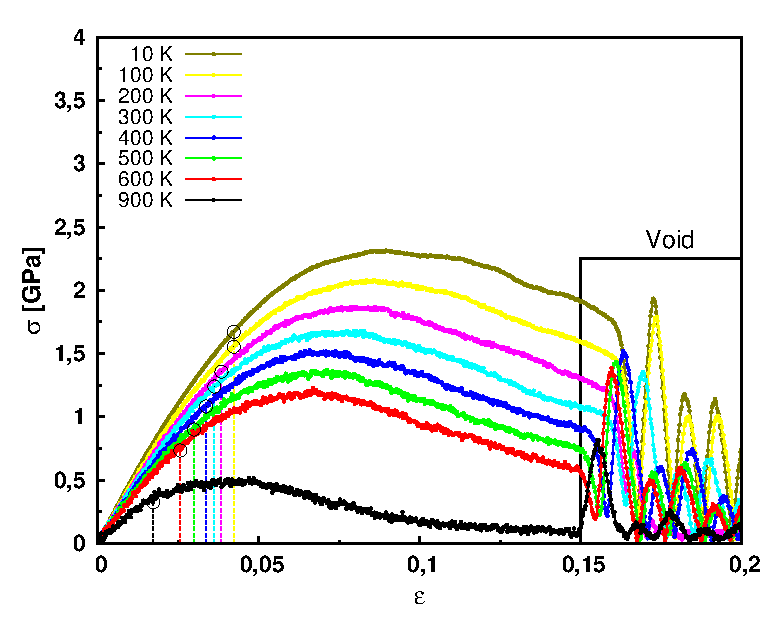
\includegraphics[width=6.3cm]{Presentacion_Mecom_2012/Tens_stress_strain_curve.eps}}
	\subfloat[Compresi\'on]{
	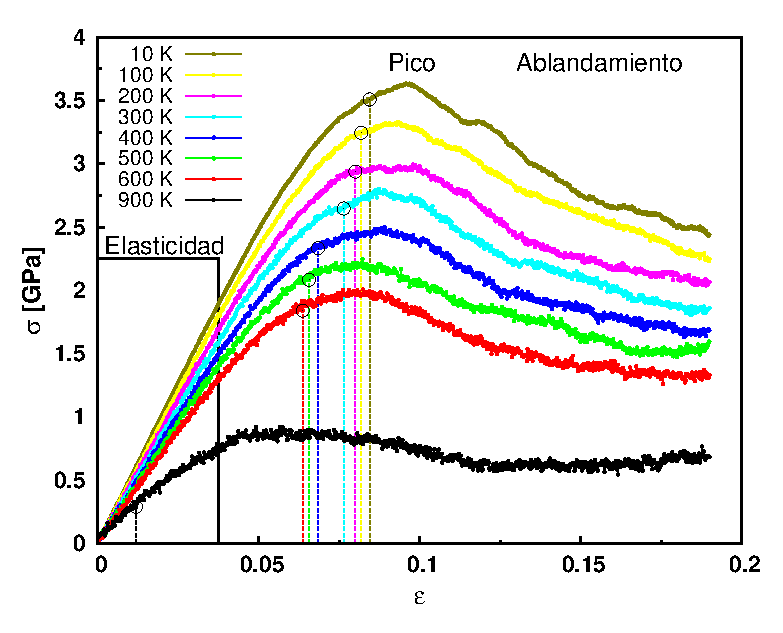
\includegraphics[width=6.3cm]{Presentacion_Mecom_2012/Comp_stress_strain_curve.eps}}
      \end{figure}
    \end{textblock*}
    \begin{textblock*}{6cm}(3.5cm,8cm) 
    \centering
      Tg=696 K\\
      (Glass transition temperature)
    \end{textblock*}
\end{frame}

\begin{frame}
 \frametitle{Resultados de las aproximaciones}
 \begin{textblock*}{6cm}(1cm,1.5cm) 
    
    \begin{table}[htp]
    \begin{center}
    \begin{tabular}{c c}
    \hline
    \textbf{Tracci\'on} & $R^{2}$ \\ \hline \hline
    Peak Von Mises stress &  0.981 \\ \hline
    Von Mises stress ($\epsilon=0.12$) & 0.998 \\ \hline
    Young Modulus & 0.990 \\ \hline
    Yield Stress &  0.972 \\ \hline
    \end{tabular}
    \end{center}
    \end{table}

    \begin{table}[htp]
    \begin{center}
    \begin{tabular}{*{4}{c}}
    \hline
    \textbf{Compresi\'on} & $R^{2}$ \\ \hline \hline
    Peak Von Mises stress & 0.997 \\ \hline
    Von Mises stress ($\epsilon=0.18$) & 0.972 \\ \hline
    Young Modulus & 0.985 \\ \hline
    Yield Stress & 0.985 \\ \hline
    \end{tabular}
    \end{center}
    \end{table}
 \end{textblock*}
  \begin{textblock*}{4.7cm}(8cm,2cm)
  \centering
   Para el c\'alculo de propiedades mec\'anicas, suponemos un comportamiento activado t\'ermicamente.
    $y=A_1^{(-T/T_0)}$
  \end{textblock*}
  \begin{textblock*}{4.7cm}(8cm,6cm)
  \centering
   El coeficiente de correlaci\'on es mayor a 0.9 en todos los casos, lo cual demuestra que la ecuaci\'on propuesta es razonable.
  \end{textblock*}
\end{frame}

\begin{frame}
 \frametitle{Gr\'aficos de las aproximaciones}
 \begin{textblock*}{10cm}(1.5cm,1cm)
 \begin{figure}[htp]
    \centering
    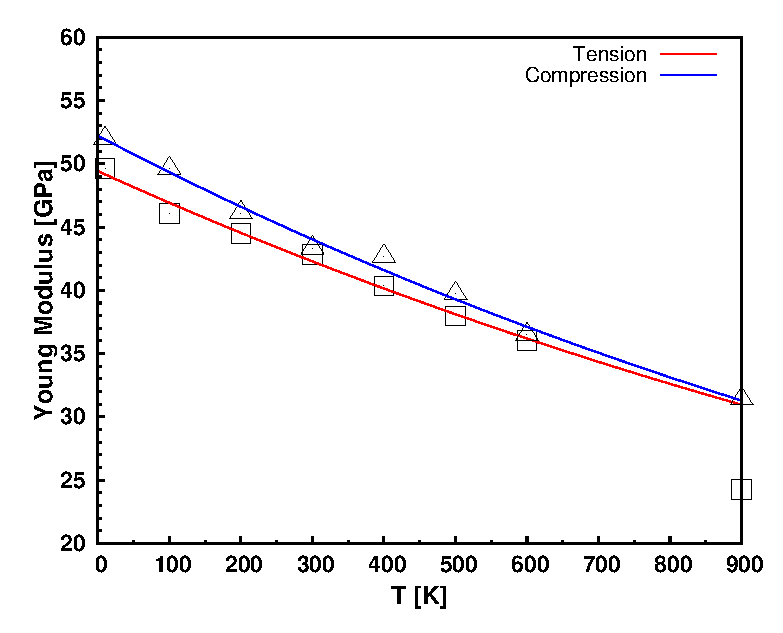
\includegraphics[width=5cm]{Presentacion_Mecom_2012/young_T_both.eps}
    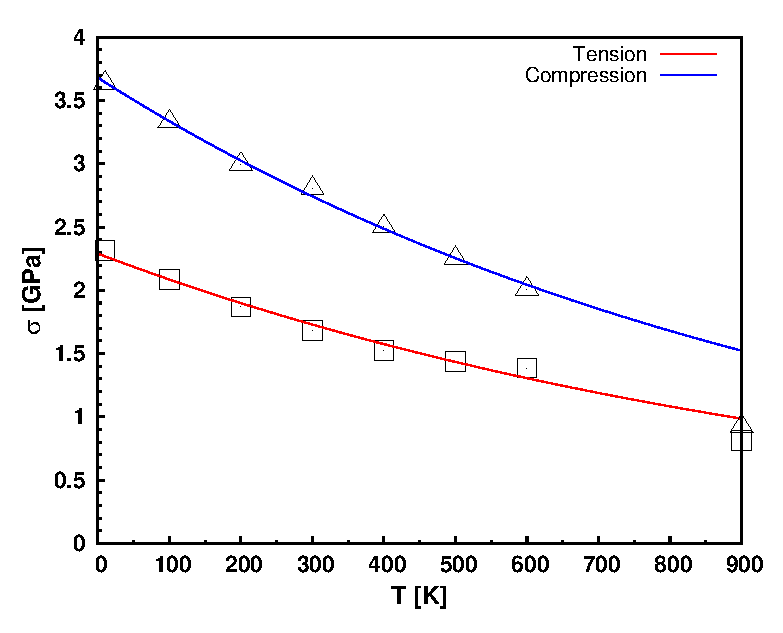
\includegraphics[width=5cm]{Presentacion_Mecom_2012/peakstress_T_BOTH.eps}
  \end{figure} 
 \end{textblock*}
 \begin{textblock*}{5cm}(1.5cm,4.9cm)
   \begin{figure}[htp]
    \centering
    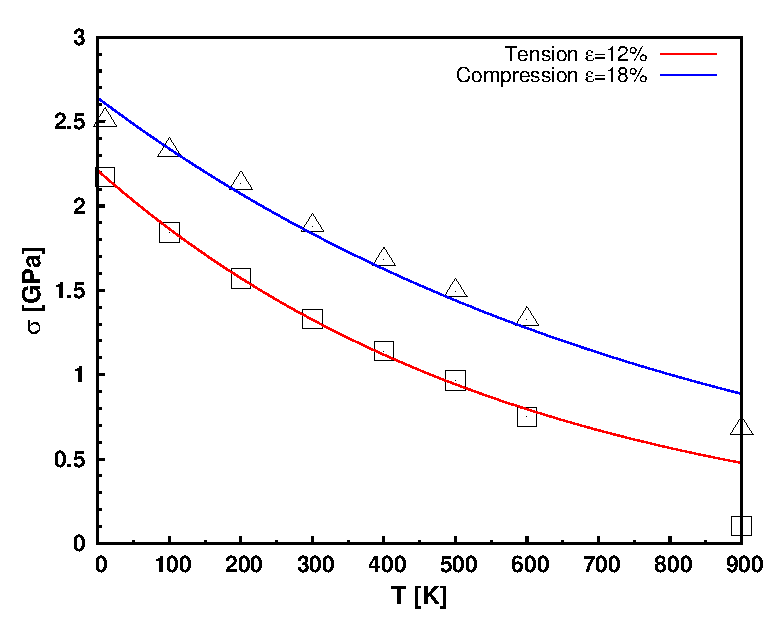
\includegraphics[width=5cm]{Presentacion_Mecom_2012/defstress_T_BOTH.eps}
  \end{figure} 
 \end{textblock*}
 \begin{textblock*}{5cm}(6.8cm,6.7cm)
  \centering
   Disminuci\'on de los valores con el aumento de temperatura.
  \end{textblock*}
\end{frame}

\begin{frame}
 \frametitle{Formaci\'on del void}
 \begin{figure}
    \centering
    \begin{tabular}{C{5cm} c}
      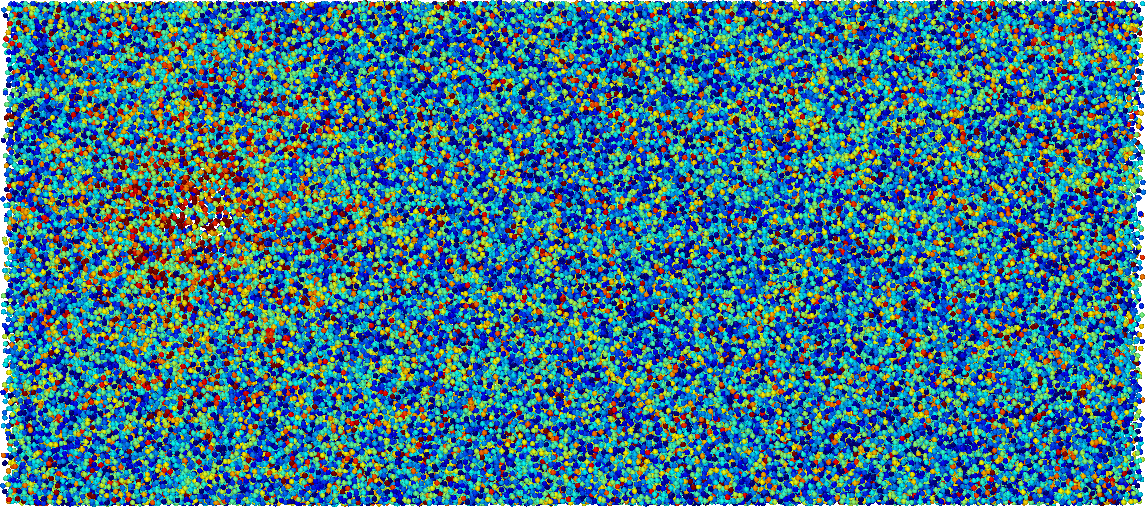
\includegraphics[width=5cm]{Cap_3/Poro_900_94000light_100-400.png} &  \multirow{3}{*}{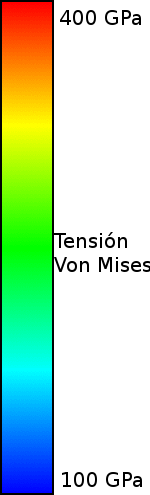
\includegraphics[width=1.2cm]{Cap_3/scale.png}}\\
      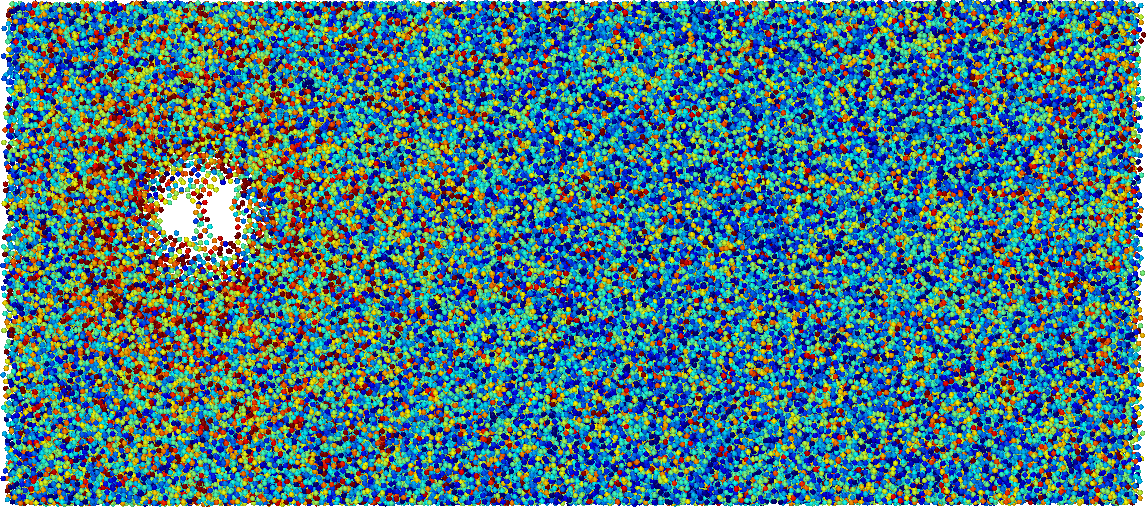
\includegraphics[width=5cm]{Cap_3/Poro_900_96000light_100-400.png} & \\
      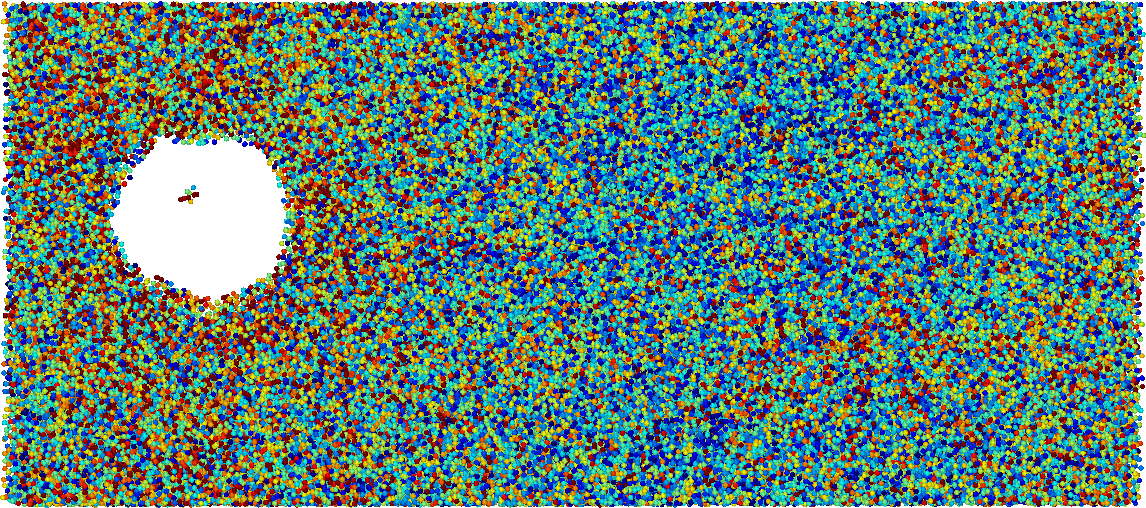
\includegraphics[width=5cm]{Cap_3/Poro_900_98000light_100-400.png} & \\
    \end{tabular}
    \label{C3:fg:voidSeq}
  \end{figure}
  \begin{textblock*}{2cm}(1cm,3cm)
      $\epsilon=14.4\%$
  \end{textblock*}
  \begin{textblock*}{2cm}(1cm,5.5cm)
    $\epsilon=14.6\%$
  \end{textblock*}
  \begin{textblock*}{2cm}(1cm,8cm)
    $\epsilon=14.8\%$
  \end{textblock*}
  \begin{textblock*}{4cm}(8.5cm,2.5cm)
    Temperatura 900K
  \end{textblock*}
\end{frame}

\begin{frame}
 \frametitle{Comportamiento pl\'astico}
 \begin{textblock*}{7cm}(0.5cm,1.4cm)
  \begin{figure}[htp]
      \centering
      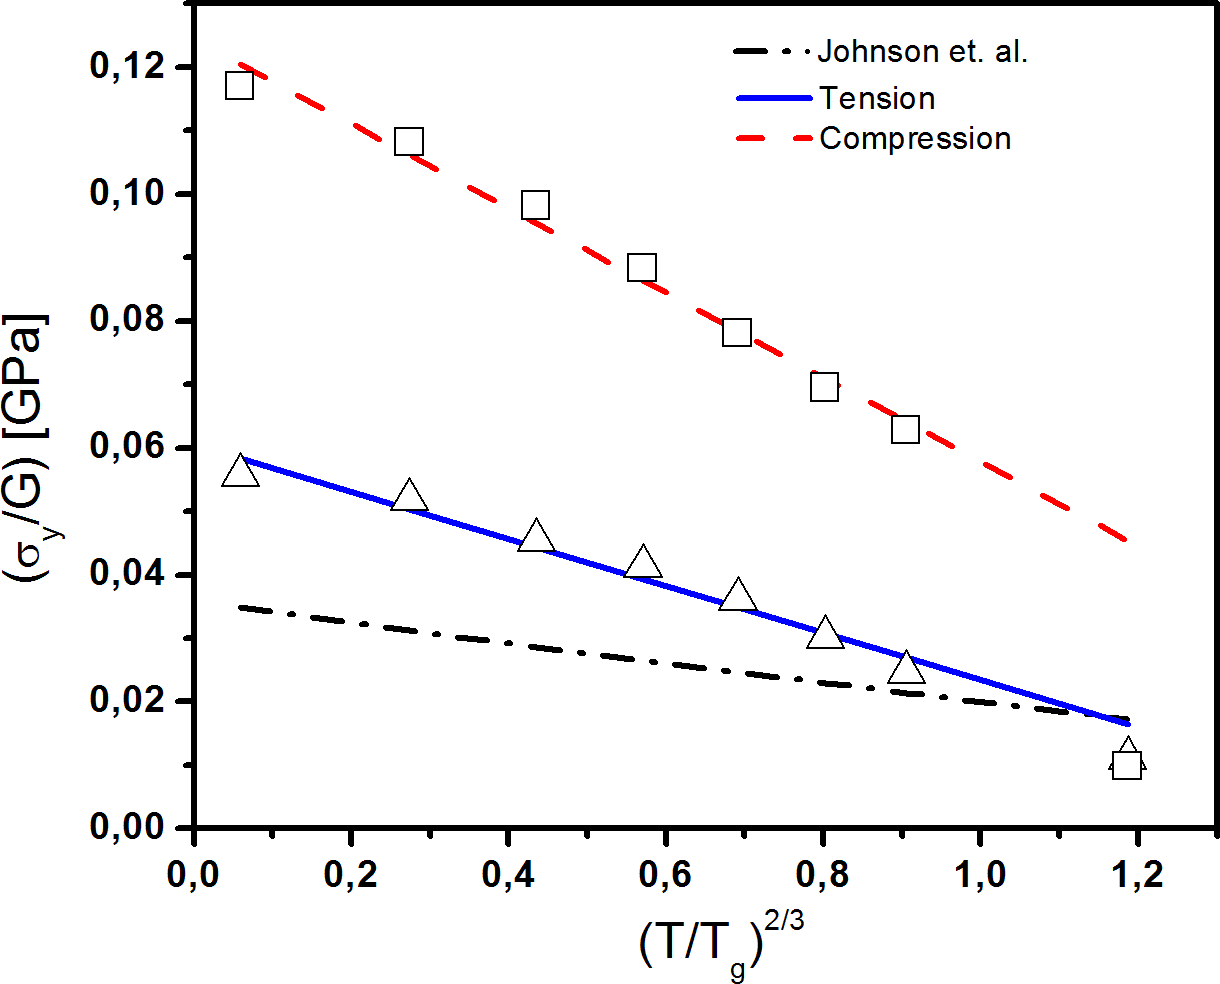
\includegraphics[width=7cm]{Presentacion_Mecom_2012/Fit2_Tercios.png}
  \end{figure}
 \end{textblock*}
 \begin{textblock*}{4.5cm}(8cm,2.5cm)
      Expresi\'on adaptada de Cheng et al. (2011) :\\
	$\sigma_y/G =A+B(T/T_g)^{2/3}$
  \end{textblock*}
  \begin{textblock*}{4.5cm}(8cm,4.5cm)
      Valores normalizados mediante:
      \begin{itemize}
       \item $T_g=696K$
       \item $G=30GPa$
      \end{itemize}
      (Johnson y Samwer, 2005)
  \end{textblock*}
  \begin{textblock*}{5cm}(2cm,6.5cm)
    \scriptsize{Esfuerzo de fluencia vs. temperatura}
  \end{textblock*}
  \begin{textblock*}{12cm}(0.5cm,8.5cm) % {block width} (coords)
    \scriptsize{Cheng Y.Q. and Ma E.. Acta Mater., 59, 1800-1807 (2011).\\
    Johnson W.L., Samwer K.. Phys. Rev. Lett., 95, 195501 (2005).}
  \end{textblock*}
\end{frame}

\begin{frame}
  \frametitle{Muestras}
  \begin{textblock*}{6cm}(0.5cm,1.5cm)
    \begin{figure}[htp]
      \centering
      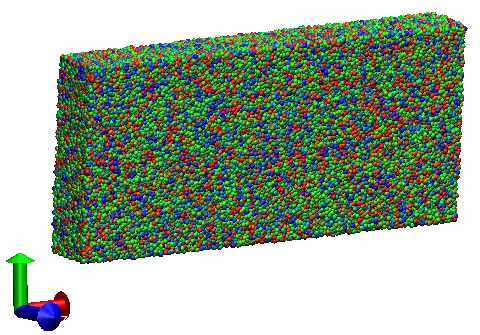
\includegraphics[width=6cm]{Cap_3/All_300K_6pstrain_sacale100-280_Trac.png}
    \end{figure}
  \end{textblock*}
  \begin{textblock*}{6cm}(6.5cm,4cm)
    \begin{figure}[htp]
      \centering
      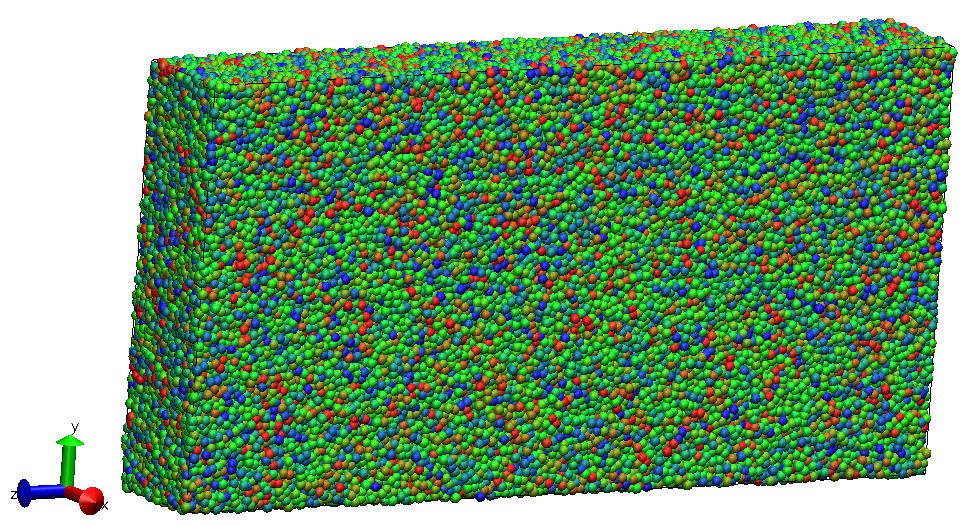
\includegraphics[width=6cm]{Cap_3/All_300K_6pstrain_sacale100-400_Comp.png}
    \end{figure}
  \end{textblock*}
  \begin{textblock*}{4cm}(3cm,6.2cm)
   \scriptsize{Tracci\'on. $T=300K$. $\epsilon=6\%$}
  \end{textblock*}
  \begin{textblock*}{5cm}(8cm,8.5cm)
   \scriptsize{Compresi\'on. $T=300K$. $\epsilon=6\%$}
  \end{textblock*}
  \begin{textblock*}{5cm}(7cm,2.5cm)
   \centering
   La escala de colores representa la tensi\'on de Von Mises
  \end{textblock*}
  \begin{textblock*}{5cm}(1cm,7.5cm)
   \centering
   No se observan bandas de corte
  \end{textblock*}
\end{frame}

\begin{frame}
  \frametitle{Deformaci\'on at\'omica}
  \begin{textblock*}{4cm}(4.5cm,1.5cm)
    \begin{figure}[htp]
      \centering
      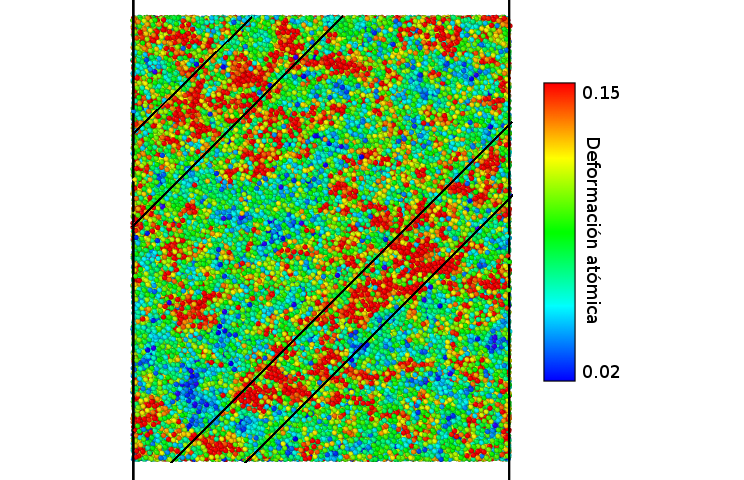
\includegraphics[height=6cm]{Cap_3/ShearBand.png}
    \end{figure}
  \end{textblock*}
  \begin{textblock*}{5cm}(6.5cm,8.5cm)
   \scriptsize{Compresi\'on. $T=300K$. $\epsilon=14\%$}
  \end{textblock*}
  \begin{textblock*}{5cm}(0.5cm,3cm)
   \centering
   La escala de colores representa deformaci\'on at\'omica
  \end{textblock*}
  \begin{textblock*}{5cm}(0.5cm,5.5cm)
   \centering
   Hay bandas de corte incipientes que se forman con una direcci\'on predominantemente diagonal
  \end{textblock*}
  
\end{frame}

\begin{frame}
  \frametitle{Resultados bajo condiciones libres}
  
  \begin{textblock*}{5cm}(0.5cm,1.2cm)
    \begin{figure}[htp]
      \centering
      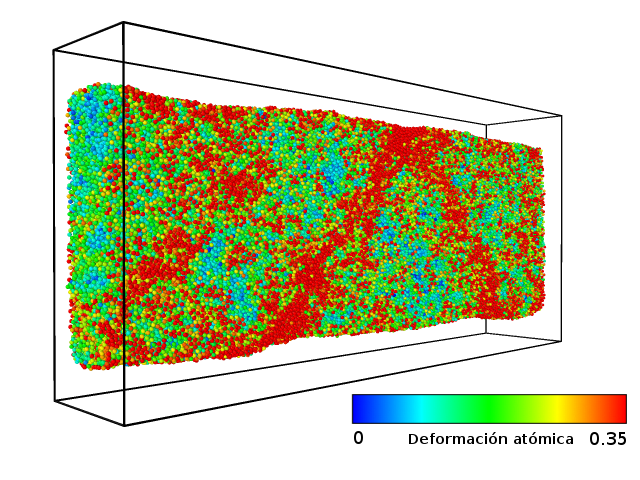
\includegraphics[width=5cm]{Cap_3/Pseudo_Free_Boundaries_ShearStrain_0_035_300K_20strain.png}
    \end{figure}
  \end{textblock*}
  
  \only<1>{
  \begin{textblock*}{5cm}(6.5cm,1.2cm)
    \begin{figure}[htp]
      \centering
      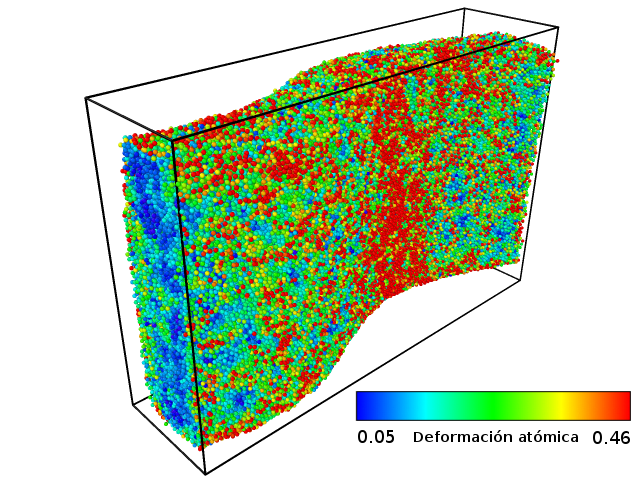
\includegraphics[width=5cm]{Cap_3/Pseudo_Free_Boundaries_ShearStrain_005_046_300K_15strain.png}
    \end{figure}
  \end{textblock*}
  }
  
  \begin{textblock*}{4cm}(2.3cm,5.5cm)
   \scriptsize{Tracci\'on. $T=300K$. $\epsilon=20\%$}
  \end{textblock*}
  
  \only<1>{
  \begin{textblock*}{4cm}(8.7cm,5.5cm)
   \centering
   \scriptsize{Compresi\'on. $T=300K$. $\epsilon=15\%$}
  \end{textblock*}
  }
  
  \begin{textblock*}{6cm}(0.2cm,6.5cm)
   \centering
   Son similares a las de nanoalambres de vidrios met\'alicos vistas en Xiao et al. (2012)\\
   Hay cambio de la secci\'on transversal en tracci\'on
  \end{textblock*}
  
  \only<1>{
  \begin{textblock*}{3cm}(6cm,5.5cm)
    \begin{figure}[htp]
	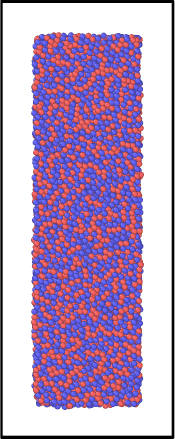
\includegraphics[width=1.3cm]{Cap_3/Pseudo_Free_Boundaries_0strain_transversal.png}
	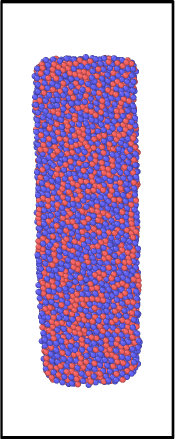
\includegraphics[width=1.3cm]{Cap_3/Pseudo_Free_Boundaries_20strain_transversal_esquina.png}
    \end{figure}
  \end{textblock*}
  }
  
  \only<2>{
  \begin{textblock*}{2cm}(8.7cm,1.8cm)
    \begin{figure}[htp]
	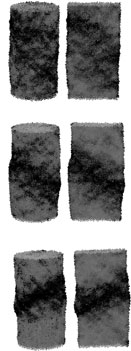
\includegraphics[width=2cm]{Presentacion_Mecom_2012/XiaoNanowire.png}
    \end{figure}
  \end{textblock*}
  
  \begin{textblock*}{6cm}(6cm,8.2cm)
    \centering
    \scriptsize{Xiao Q., Sheng H.W. and Shi Y.. MRS Communications, 2, 13-16 (2012)}
  \end{textblock*}

  \begin{textblock*}{2cm}(6.7cm,3.1cm)
    \centering
    \scriptsize{$1.7\cdot10^{12}K/s$}
  \end{textblock*}
  
  \begin{textblock*}{2cm}(6.7cm,4.9cm)
    \centering
    \scriptsize{$1.7\cdot10^{11}K/s$}
  \end{textblock*}
  
  \begin{textblock*}{2cm}(6.7cm,6.8cm)
    \centering
    \scriptsize{$1.7\cdot10^{10}K/s$}
  \end{textblock*}
  
  }
\end{frame}